\chapter[Particle Identification and Event Reconstruction]{Particle Identification and Event Reconstruction}
\label{chap:ParticleID}

\section{Jets Identification}
\label{sec:Jet}


% Jets are reconstructed with the Particle Flow technique (PF) using the anti$-$k$_{T}$ algorithm \cite{Alwall:2011uj}. 
The PF technique \cite{ParticleFlow} takes the information collected by the CMS subdetectors in order to identify and reconstruct 
all the vissible final-state particles (electrons, muons, photons, charged hadrons and neutral hadrons) produced 
in the hard interaction. The PF technique reconstructs the jet constituents individually from the 
combination of tracks and calorimeter clusters. Then, the jet reconstruction is performed 
with the anti$-$k$_{T}$ algorithm \cite{AntiKTAlgorithm} iterating over all the PF objects, using a distance parameter of 
$\Delta R = 0.4$ in the $\eta-\phi$ plane, where $\Delta R = \sqrt{(\Delta \phi)^2+(\Delta \eta)^2}$.\\

\begin{figure}%[!Hhtbp]
  \begin{center}
    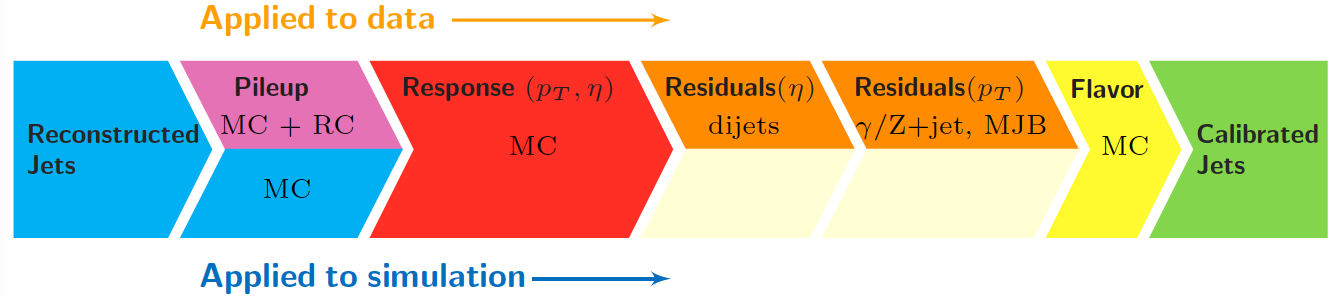
\includegraphics[width=0.9\textwidth]{figuras/Chapter3/JEC_levels.png}
    \caption{Levels of corrections for PF jet four-momentum. Figure taken from \cite{JESandJER}}
    \label{fig:JEC_levels}
  \end{center}
\end{figure}

The four-momentum of the reconstructed jet is the addition of the four-momenta of all the PF objects associated to the jet. However
due to detector responses and experimental effects, the PF jet four-momentum does not correspond to the four-momentum
at parton or hadron level; therefore, jet energy corrections (JEC) are required. Figure \ref{fig:JEC_levels} shows the different 
levels of corrections which are applied in a fixed sequence. Each correction corresponds to a multiplicative factor $C$ on 
the PF jet four-momentum ($p_{\mu}^{raw}$):

\begin{equation}
 p_{\mu}^{corrected} = C \times p_{\mu}^{raw}
\end{equation}

The first step in the chain is the ``L1 corrections'' (also refered as ``pileup offset''). It attends the additional tracks and the excess of energy deposits 
in the calorimeters due pile-up events . The amount of the pile-up contribution 
to the jet energy can be estimated from the global per-event $p_{T,offset}$ density $\rho$ and the jet area \cite{JECpileup}. This amount 
is obtained from simulated dijet events with and without PU. \\

The second level of JEC is related with the detector response to hadrons (L2L3 MC-truth corrections), correcting 
the non-uniformity in $\eta$ and the non-linearity in $p_{T}$. The simulated jet response is determinated
with QCD-multijet events generated with Pythia and with a simulation of the CMS detector based
on Geant4.\\

After these steps, the L2L3 Residual corrections are applied in order to address the remaining difference 
between the jet response on data and MC (of the order of $1 \%$). This corrections are achieved with data-driven methods, using 
dijet samples for $\eta$-dependent corrections and $\gamma /$Z+jets samples for the corrections to $p_{T}$. The last stage 
of the JEC (L5) is optional and it accounts the jet-flavor corrections. \\

%An efficiency larger than 80% is obtained for jets with a p T > 20 GeV/c. The 100% plateau is reached above
%40 GeV/c, at which point the mismatched jet rate is negligible





%JER Article
%The jet p T resolutions are determined with both dijet and photon+jet events, as discussed in
%section 8. The reference resolutions obtained from simulation are parameterized as a function of
%particle-level jet p T, ptcl (defined in section 2) and average number μ of pileup interactions in bins
%of jet η. Corrections for differences between data and MC simulation are applied as η-binned scale
%factors




%Since in average 85 $\%$ of the constituents of a jet are charged particles and photons, the jet energy resolution

%PF jet momentum and spatial resolutions are greatly improved with respect to calorimeter jets, as
%the use of the tracking detectors and high granularity of the ECAL improves the energy resolution
%through the independent measurements of charged hadrons and photons inside a jet, which together
%2.1constitute ≈85% of the average jet energy. In reconstructing the PF candidate four-momentum,
%photons are assumed massless and charged hadrons are assigned the charged pion mass.

%As mentioned previously, the typical jet energy fractions carried by charged particles, photons
%and neutral hadrons are 65%, 25% and 10% respectively. These fractions ensure that 90% of
%the jet energy can be reconstructed with good precision by the particle-flow algorithm, both in
%value and direction, while only 10% of the energy is affected by the poor hadron calorimeter
%resolution and by calibration corrections of the order of 10 to 20%. As a natural consequence,
%it is expected that jets made of reconstructed particles be much closer to jets made of MonteCarlo–generated
%particles than jets made from the sole calorimeter information, in energy, direction
%and content. It is the purpose of this section to quantify this statement.

%($c\tau > 1$ cm) 


%\subsection{Online Identification}
%\label{subsec:JetTrigger}

%\subsection{Offline Identification}
%\label{subsec:JetReconstruction}

\section{Electron Identification}
\label{sec:Electron}

%\subsection{Online Identification}
%\label{subsec:ElectronTrigger}

%\subsection{Offline Identification}
%\label{subsec:ElectronReconstruction}

\section{Muon Identification}
\label{sec:Muon}

\section{B-Jet Identification}
\label{sec:BJet}

\section{MET}
\label{sec:MET}

\section{Tau Lepton}
\label{sec:Tau}

\subsection{Tau Identification}
\label{subsec:TauTrigger}

\subsection{Tau Reconstruction}
\label{subsec:TauReconstruction}

\subsection{Working Points}
\label{subsec:wp}

\subsubsection{Efficiency of Working Points}
\label{subsubsec:Eff_WP}

\subsection{Fake Rates}
\label{subsec:FakeRates}

\subsection{Perspectives Run III}
\label{subsec:Perspectives}